
%%%%%%%%%%%%%%%%%%%%%%%%%%%%%%%%%%%%%%%%%%%%%%%%%%%%%%%%%%%%%%%%%%%%%%%%%%%%%%%%%%%%%%%%%%%%%%%%%%%%%%%%%%%%
%%%%%%%%%%%%%%%%%%%%%%%%%%%%%%%%%%%%%%%%%%%%%%%%%%%%%%%%%%%%%%%%%%%%%%%%%%%%%%%%%%%%%%%%%%%%%%%%%%%%%%%%%%%%
%
% new section
%
%%%%%%%%%%%%%%%%%%%%%%%%%%%%%%%%%%%%%%%%%%%%%%%%%%%%%%%%%%%%%%%%%%%%%%%%%%%%%%%%%%%%%%%%%%%%%%%%%%%%%%%%%%%%
%%%%%%%%%%%%%%%%%%%%%%%%%%%%%%%%%%%%%%%%%%%%%%%%%%%%%%%%%%%%%%%%%%%%%%%%%%%%%%%%%%%%%%%%%%%%%%%%%%%%%%%%%%%%
\chapter{Conjugate Heat Transfer in Solid Breeder Pebble Beds with Lattice-Boltzmann Modeling}\label{sec:modeling-lbm}
The volume-averaged approach of the CFD-DEM coupling is an effective and efficient method for solving transiently-coupled heat transfer between flowing helium and pebble beds \textit{via} volume-averaging techniques to handle the fluid conservation equations. However, the approach does not provide a complete view of the tortuous flow of interstitial helium because the CFD-DEM solver does not resolve the helium pathways on the particle scale. Therefore we have also investigated fluid-pebble interactions by means of linking DEM pebble beds with lattice-Boltzmann solvers which allows us the ability to solve the complete conjugate heat transfer of flowing helium through pebble beds within reasonable computational times.

The lattice-Boltzmann method (LBM) to simulate fluid flow is a growing field of numerical modeling with a rich historical development. As the LBM approach is relatively new and its governing equations have roots in both computer science and statistical mechanics, in this section I will first review notable evolutions in modeling history and the background physics leading to the governing equations -- which lend themselves to relatively straightforward numerical implementation. References~\cite{Chen1998a,Viggen2009,Sukop2007,Chopard2002,succi2001lattice} provide more thorough descriptions of the physics, modeling approaches, and applications of LBM theory to fluid dynamics problems.

\section{Historical Development and Physics of LBM}
We begin with a brief discussion of the Boltzmann equation describing the statistical behavior of non-equilibrium thermodynamic systems. Then we will introduce some of the lattice gas automata predecessors to the current lattice-Boltzmann method.

\subsection{Discretized Boltzmann Equation}\label{sec:lbm-intro}

In the realm of statistical mechanics, suppose we wish to know, at a certain time $t$, how many particles exist at a given location, $\vec{x}$, that have momentum, $\vec{p}$. We define a number,
\begin{equation}
	n = f(\vec{x},\vec{p},t)\mathrm{d}\vec{x}\mathrm{d}\vec{p}
\end{equation}
as the number of $n$ particles in the system that exist within the coordinates of $\mathrm{d}\vec{x}$ and momenta $\mathrm{d}\vec{p}$ at that instant. $f(\vec{x},\vec{p},t)$ is the probability density function representing the odds of finding a particle per phase space ($\vec{x},\vec{p}$) at a moment in time, $t$.

Now let us assume we apply a small force, $\vec{F}$, to all the $n$ particles and then increment time by $\mathrm{d}t$. Assuming further that none of the particles collide (with each other or any other particles in the system), the particles will have moved an amount $\vec{x} + \frac{\vec{p}}{m}\mathrm{d}t$. The particles will all also have had their momentum changed by an amount $\vec{p} + \vec{F}\mathrm{d}t = \vec{p} + \mathrm{d}\vec{p}$. In other words, those $n$ particles are now found in the phase space of
\begin{equation}
 	n = f(\vec{x} + \frac{\vec{p}}{m}\mathrm{d}t,\vec{p} + \mathrm{d}\vec{p},t + \mathrm{d}t)\mathrm{d}\vec{x}\mathrm{d}\vec{p}
 \end{equation}

The number of particles in the two moments of time are conserved, so we can also say
\begin{equation}
	f(\vec{x} + \frac{\vec{p}}{m}\mathrm{d}t,\vec{p} + \mathrm{d}\vec{p},t + \mathrm{d}t)\mathrm{d}\vec{x}\mathrm{d}\vec{p} = f(\vec{x},\vec{p},t)\mathrm{d}\vec{x}\mathrm{d}\vec{p}
\end{equation}

Next we relax the assumption of no collisions. If we focus our attention of the phase space as before, some of the particles that began at $(\vec{x},\vec{p},t)$ will not arrive at the phase space of $(\vec{x} + \frac{\vec{p}}{m}\mathrm{d}t,\vec{p} + \mathrm{d}\vec{p},t + \mathrm{d}t)$. By the same measure, some particles that began in some other phase space \textit{will} arrive in $(\vec{x} + \frac{\vec{p}}{m}\mathrm{d}t,\vec{p} + \mathrm{d}\vec{p},t + \mathrm{d}t)$. Now the number of particles is not conserved and we write the net number of particles having left/entered this phase space as
\begin{equation}
	\Omega\mathrm{d}\vec{x}\mathrm{d}\vec{p}\mathrm{d}t
\end{equation}
where $\Omega$ is classically referred to as the collision operator. This function dictates the evolution of particles after a collision (what phase space they leave/enter). Treatment of the collision operator is itself a source for discussion but we leave it as a generic operator. Thus the balance of particles is now
\begin{equation}\label{eq:particle-balance}
	f(\vec{x} + \frac{\vec{p}}{m}\mathrm{d}t,\vec{p} + \mathrm{d}\vec{p},t + \mathrm{d}t)\mathrm{d}\vec{x}\mathrm{d}\vec{p} - f(\vec{x},\vec{p},t)\mathrm{d}\vec{x}\mathrm{d}\vec{p} = \Omega\mathrm{d}\vec{x}\mathrm{d}\vec{p}\mathrm{d}t
\end{equation}

To be precise, to arrive at the collision operator, $\Omega$, in the form we have used in \Cref{eq:particle-balance}, it is required to make a few more assumptions on the system. Following Ludwig Boltzmann, we assume: the particles are dilute, point-like, and structureless that only interact \textit{via} short-range two-body potentials. Another famous assumption from Boltzmann was of \textit{Stosszahlansatz} (molecular chaos) which allow the inter-particle interactions to be described only in terms of their local binary collisions with very long paths through free space between collisions.\cite{succi2001lattice} For the sake of this discussion, we will just accept the formulation of \Cref{eq:particle-balance} as the evolution equation for the particles in our system. 

% As a side note, after taking a multi-dimensional Taylor expansion of \Cref{eq:particle-balance}, we arrive at the the recognizable Boltzmann equation,
% \begin{equation}\label{eq:boltzmann-continuum}
% 	\left[\vec{c}\cdot\nabla + \vec{F}\cdot\partial_\vec{p}  + \partial_t\right] f(\vec{x},\vec{p},t) = \Omega
% \end{equation}
% where $\vec{c} = \vec{p}/m$. In the form of \Cref{eq:boltzmann-continuum}, it is clear how the Boltzmann equation describes the evolution in a continuous way. There are an infinite number of directions and momenta for the particles to evolve into/from. 

We consider a case where there are a discrete number of directions a particle may travel, such as toward discrete $i$ directions of neighboring nodes in a lattice. In such a case, velocities point only toward those neighbors, $\vec{c}\rightarrow\vec{c}_i$. In \Cref{eq:particle-balance}, we also normalize the mass such that $m=1$, making $\vec{p}/m = \vec{p}=\vec{c}$. In discrete increments of time, we also write the collision operator in a discrete form, $\Omega\mathrm{d}t \rightarrow \Omega_i(\vec{x},t)$. Thus, \Cref{eq:particle-balance} becomes,
\begin{equation}
	f_i(\vec{x}+\vec{c}_i\Delta t, t + \Delta t) - f_i(\vec{x},t) = \Omega_i(\vec{x},t)
\end{equation}

Lastly, if we assume that we are using time units that have also been normalized such that $\Delta t = 1$, the above becomes
\begin{equation}\label{eq:boltzmann2lbe}
	f_i(\vec{x}+\vec{c}_i, t + 1) - f_i(\vec{x},t) = \Omega_i(\vec{x},t)
\end{equation}

In the form of \Cref{eq:boltzmann2lbe}, our discretized version of the Boltzmann equation for statistical mechanics will be seen to be identical to a lattice-based formulation that will be arrived at purely from the point of view of lattice gas automatons.



\subsection{Lattice Gas Automata}

In a broad sense, lattice gas automata (LGA) simulated the behavior of individual particles with a simple boolean approach where basic collision rules were defined at nodes in a lattice. As particles approach nodes from neighbors at a given time, rules dictate the direction of the particle at the next moment in time. Computationally, the particles were simply represented with boolean operators that said either 1: a particle existed at that node in that direction; or 0: no particle existed at that node in that direction. Conceptually, the particles can be thought of as hard spheres that would collide on nodes of a lattice; collisions would send the particles rebounding along discrete directions toward neighboring nodes. The restraint on collision rules required that they obey conservation of mass and momentum. 

The earliest LGA was a two-dimensional model by Hardy, Pomeau, and de Pazzis (HPP) in 1973.\cite{Hardy1975} The HPP model applied basic conservation rules that particles had to obey at each node. From the streaming particles, macroscopic units could be extracted. For instance, the particle density at a node is found from the total number of boolean particles at that node,
\begin{equation}
	\rho(\vec{x},t) = \sum_i n_i(\vec{x},t)
\end{equation}
where $n_i(\vec{x},t)$ are the particles occupying the node at $\vec{x}$ at time $t$ with a velocity of $\vec{c}_i$. As mentioned, the value of $n$ is a boolean value of 1 or 0 if the particle is present or not, respectively. Similarly, the momentum at the node is found as,
\begin{equation}
	\rho(\vec{x},t)\vec{u}(\vec{x},t) = \sum_i \vec{c}_in_i(\vec{x},t)
\end{equation}
where $\vec{u}(\vec{x},t)$ is the mean velocity of the particles at the node at that time.

Boolean nature of the HPP automata meant that the solution was not only exact (not susceptible to any round-off errors of floating point numbers) but each node required only four bits to completely describe the state (each bit described the four directions of traveling particles in the two dimensional node).\cite{Hardy1975} Furthermore, the HPP model benefited from the inherently parallel nature of all LGA simulations. The collision behavior at any given node is independent of all other nodes; the nodes only need to communicate when particles stream to neighbors.\cite{succi2001lattice}

The LGA method was given considerable more attention after 1986 when Frish, Hasslacher, and Pomeau (FHP) showed it to be possible to solve lattice gas automata simulations that were ostensibly equivalent to Navier-Stokes equations (in two dimensions).\cite{Frisch1986} Descriptions of the hexagonal lattice used in the FHP model can be found in the textbooks of Succi\cite{succi2001lattice} and Sukop \& Thorne\cite{Sukop2007}. The FHP method gave qualitatively beautiful reproductions of hydrodynamic phenomena.

Other such LGA models were developed with the same fundamental construction as the two models mentioned here. All the models followed the same basic form of evolution of the particles. Following the form of Ref.~\cite{chopard1998cellular},
\begin{equation}\label{eq:lattice-evolution}
	n_i(\vec{x}_i + \vec{c}_i,t+1) - n_i(\vec{x},t) = \Omega_i(\vec{x},t)
\end{equation}
where, in lattices, $\Delta t = 1$ is a standard normalization. After already deriving the Boltzmann equation, \Cref{eq:lattice-evolution} should appear quite familiar. The equation states that the particle occupation number at a specific location and time, $n_i(\vec{x},t)$, evolves based on the collision rules, $\Omega_i(\vec{x},t)$, defined at every node, $\vec{x}$. In the LGA framework, the collision operator is much simpler than the form used in the Boltzmann equation for statistical mechanics. Here, the rules are simplified and discretized so that $\Omega_i$ can exist in a simple look-up table or explicit function of $n_i$ (with randomness).\cite{chopard1998cellular,Sukop2007}

Collision operators are chosen such that they obey conservation of mass and momentum, expressed as,
\begin{subequations}
\begin{align}
	\sum_i\Omega_i &= 0\\
	\sum_i\vec{c}_i\Omega_i&=0
\end{align}
\end{subequations}

With these simple rules applied to specific lattices, such as the LHP hexagons, it is possible to show the lattice gas automata, on a proper lattice, can be re-expressed to satisfy continuity and conservation of momentum (see Ref.~\cite{Viggen2009,Frisch1986}). The construction of LGA schemes were extremely simple yet, with their connection to conservation equations in the continuum, seemed promising as a perfect scheme for modeling fluid mechanics.

However, as exciting as the early LGA methods were, their drawbacks were very nearly as disheartening after being formally compared to the Navier-Stokes equations. Succi provides a thorough summary of the early issues with FHP (and all LGA approaches).\cite{succi2001lattice} For the sake of brevity we only mention that the main disadvantages were: lack Galilean invariance at higher Mach numbers (the results were not the same irrespective of inertial frame) and statistical noise in macroscopic quantities. The microscopic nature of LGAs -- tracking the paths of individual particles -- precluded the method from ever completely eliminating the issues such as statistical noise. The solution to the issues came in 1988 as a group zoomed-out from the microscopic into a mesoscopic formulation -- the first version of what would eventually be the lattice-Boltzmann numerical method.



\subsection{The Lattice-Boltzmann Equation}\label{sec:lbm-equations}

McNamara and Zanetti proposed a fix to the statistical noise in LGA \textit{via} ensemble-averaging the boolean occupation numbers,\cite{McNamara1988}
\begin{equation}\label{eq:lbm-pdf}
	f_i = \langle n_i \rangle = \frac{1}{q}\sum_{i=1}^qn_i
\end{equation}
where $q$ is the number of lattice directions from the node. The average quantity, $f_i$, was now identical in form to the distribution function of the Boltzmann equation. In the formulation of McNamara and Zanetti, we are no longer tracking individual boolean particles but a representative ensemble population of the particles.

Replacing the boolean occupation numbers in \Cref{eq:lattice-evolution} with the density function of \Cref{eq:lbm-pdf}, we have
\begin{equation}\label{eq:lbm-evolution}
	f_i(\vec{x}+\vec{c}_i, t + 1) - f_i(\vec{x},t) = \Omega_i(\vec{x},t)
\end{equation}
which is precisely the form found for the discretized Boltzmann equation in \Cref{eq:boltzmann2lbe}! This is the essence of the lattice-Boltzmann method: it can be considered as a simplification of the Boltzmann concept \textit{via} reduction of the continuous phase space into a finite number of discrete phase options; or it similarly can be considered as an ensemble-averaging of the lattice gas automata into calculations of mesoscopic distribution functions.

The boolean occupation numbers were simply imagined as the actual particles traveling from node to node in the LGA lattice. The ensemble average of these numbers, $f_i(\vec{x},t)$, akin to the probability density function from kinetic theory, can be envisioned to be the probability of finding a density of particles pointing in a certain direction, $i$, at a given node, $\vec{x}$, at a specific point in time, $t$. The values of $f_i$ are direction-specific fluid densities and thus macroscopic fluid properties are still directly calculated from them,
\begin{subequations}\label{eq:lbm2physical}
\begin{align}
	\rho(\vec{x},t) &= \sum_i f_i(\vec{x},t)\\
	\vec{u}(\vec{x},t) &= \frac{1}{\rho(\vec{x},t)}\sum_i \vec{c}_if_i(\vec{x},t)
\end{align}
\end{subequations}

The fluid pressure is related to the density for an ideal gas, so we can find the physical pressure in terms of the lattice density,
\begin{equation}
	p = p_0\frac{\rho(\vec{x},t)}{\rho_0}
\end{equation}

The density distribution function, while eliminating statistical noise, broke the exactness of calculations from the boolean numbers of $n_i$ in LGA methods. The density distribution function is now a floating point number, requiring more memory storage per node and introducing round-off error into calculations. In Chapter 3 of Ref.~\cite{succi2001lattice}~, Succi provides an excellent discussion of the early stages of LBM and the problems that the early models (such as those of McNamara and Zanetti) faced as well as their many great advantages. For our purposes, we accept \Cref{eq:lbm-evolution} as the fundamental equation driving the evolution of the density distribution function in a system.



\subsubsection{Collision Operator for Lattice-Boltzmann Equation}

The strength of \Cref{eq:lbm-evolution} hinges on the ability for the collision operator, $\Omega_i(\vec{x},t)$, to allow reproduction of the Navier-Stokes equations. Up to this point we have only alluded to its function in the LGA and now LBM computations. While there are many potential collision operators (see Ref.~\cite{succi2001lattice}), we focus on the operator proposed by Qian, d’Humieres, and Lallemand.\cite{qian1992lattice} Noting the similarities of LBM to kinetic theory, Qian, d'Humieres, and Lallemand proposed a collision operator similar in form to that proposed by Bhatnagar, Gross, and Krook in 1954 for the Boltzmann equation.\cite{Bhatnagar1954a} Thus the operator was named the BGK collision operator and is given as,
\begin{equation}\label{eq:bgk-operator}
	\Omega_i = -\frac{1}{\tau}\left[f_i(\vec{x},t) - f_i^\eq(\vec{x},t)\right]
\end{equation}
where $\tau$, a free parameter, is the relaxation time of the lattice, and $f_i^\eq$ is the equilibrium distribution. Thus in the BGK formulation, the collision operator is a relaxation of the node towards equilibrium for the density distribution function.\cite{Bhatnagar1954a}

Inserting the operator of \Cref{eq:bgk-operator} into the evolution of the density distribution function, \Cref{eq:lbm-evolution}, we have the lattice-Boltzmann evolution equation with the BGK operator,
\begin{equation}\label{eq:lbm-bgk}
	f_i(\vec{x}+\vec{c}_i, t + 1) = f_i(\vec{x},t) - \frac{1}{\tau}\left[f_i^\eq(\vec{x},t) - f_i(\vec{x},t)\right]
\end{equation}

In spite of the relaxation time being a free parameter, there are limits to its value. The kinematic viscosity in a lattice is,
\begin{equation}\label{eq:lbm-viscosity-relaxation-time}
	\nu = c_s^2\left(\tau-\frac{1}{2}\right)
\end{equation}
which shows that $\tau$ can not shrink to an arbitrarily small number. Numerical instabilities appear as $\tau \rightarrow 0.5$ and the kinematic viscosity $\nu \rightarrow 0$. Furthermore, if $\tau > 1$, we have subrelaxation and the distribution function will never completely relax to equilibrium. When $\tau < 1$, we have overrelaxation and the system out of equilibrium will advance toward it at different rates. When $\tau$ is small, the relaxation to $f^\eq$ is fast and thus the viscosity of the lattice can be considered to be small. A negative viscosity occurs if $\tau < 1/2$ and is not allowed.\cite{Chopard2002,Chen1998a}

The equilibrium distribution function, $f^\eq$, is derived from the Maxwell-Boltzmann velocity distribution in statistical mechanics. With clever application of the ideal gas law and the isothermal ideal gas pressure relation (see, for example, Refs.~\cite{Viggen2009,Chopard2002}), it is possible to find an equilibrium distribution that allows $\Omega_i$ to respect all conservation laws,
\begin{equation}\label{eq:equilib-dist-function}
	f_i^\eq = \rho(\vec{x},t)w_i\left[1+\frac{\vec{u}\cdot\vec{c}_i}{c_s^2} + \frac{(\vec{u}\cdot\vec{c}_i)^2}{2c_s^4} - \frac{\vec{u}^2}{2c_s^2} \right]
\end{equation}
where $c_s$ is the speed of sound on the lattice and $w_i$ are weighted lattice constants. In the development of the equilibrium function, it is assumed that the velocity of the fluid is small compared to the speed of sound on the lattice, in other words we require small Mach numbers: $\Ma = \frac{|u|}{c_s} < 1$, on the lattice.\cite{qian1992lattice,Chen1998a} It is worth noting here that the equilibrium function of \Cref{eq:equilib-dist-function} is defined entirely in terms of local velocity and density; everything is in terms of node $i$ and no other neighboring node. This feature aids the LBM approach in being highly parallelizable in the same way the LGA method was.

There are several conditions a lattice must meet to satisfy the isotropy necessary to regain the Navier-Stokes equations in the macroscopic form.\cite{Viggen2009,Latt2007} A lattice structure in $d$ dimensions with $q$ lattice directions is commonly identified with the D$d$Q$q$ lattice label. In the three-dimensional flow of our packed beds, we use the D3Q19 lattice, \textit{i.e.} $d=3$ dimensions, and $q=19$ nodes surround the node of interest (including the node itself). A representative node from the D3Q19 lattice is shown in \Cref{fig:d3q19-lattice}.
\begin{figure}[t]
	\centering
	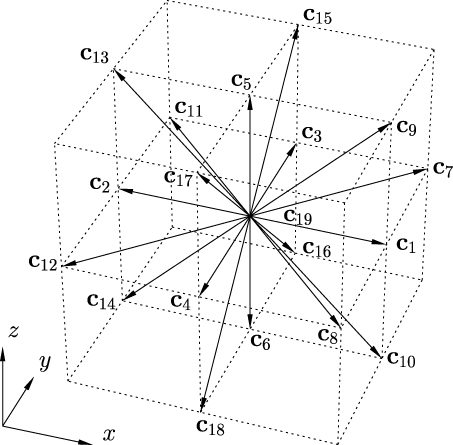
\includegraphics[width=\singleimagewidth]{figures/lbm/4193301.jpg}
	\caption{A representative node with directional vectors to the 18 neighbors (+1 central node) in the D3Q19 lattice (reproduced from Ref.~\cite{1742-5468-2010-01-P01018}).}\label{fig:d3q19-lattice}
\end{figure}

The numbered directions in the lattice of \Cref{fig:d3q19-lattice} follows the standard practice of LBM. The index $i=0$ corresponds to the node center. The indices $i = 1,2,3,\dots,6$ point to the six faces of the cube surrounding the node. Lastly, the indices $i=7,8,9,\dots,18$ point to the twelve midpoints of the edges of the cube. The weight constants, satisfying lattice symmetry, of the lattice structure of \Cref{fig:d3q19-lattice} are calculated in Ref.~\cite{Latt2007} and given as,
\begin{equation}\label{eq:d3q19-weights}
	w_i = \begin{cases}
	\frac{1}{3}			& i = 0\\
	\frac{1}{18} 		& i = 1,2,3,\dots,6\\
	\frac{1}{36}		& i = 7,8,9,\dots,18
	\end{cases}
\end{equation}

The lattice weights, $w_i$ are necessary to account for the different vector lengths in the lattice. In principle, there is freedom in choosing the lattice speed of sound, $c_s$, requiring a change to the rest-weight of $w_0$ to maintain lattice symmetry. However, in practice, it is common to use $c_s^2 = \frac{1}{3}$ for numerical stability.\cite{Latt2007,succi2001lattice}.




\subsubsection{Boundary Conditions}
Techniques for implementation of no-slip boundary conditions in LBM are direct descendants of the bounce-back schemes from lattice gas automata. In the scheme, lattice nodes that exist at the boundary have particle directions that point into the wall. For example, see $f_4$, $f_7$, and $f_8$ in \Cref{fig:wall-lattice-bc} for a D2Q9 lattice. The scheme is `bounce-back' because as particles stream into the wall, their distributions are scattered back in equal and opposite directions. Computationally, the bounce-back scheme is very attractive for the simplicity of implementing the method even in complex geometries. A fact which makes the use in LBM particularly attractive for packed bed simulations.\cite{Chen1998a} The bounce-back scheme has been shown to be first-order accurate for most three-dimensional flows, degrading the other-wise second order accuracy of the fluid bulk calculations.\cite{Zou1997,Chen1998a} To combat the loss in accuracy with increasing Reynolds number, several modifications to the bounce-back scheme have been proposed.\cite{Chen1998a} However, for the porous flow to be studied in ceramic pebble beds, it suffices to implement the bounce-back boundary condition to enforce no-slip at the fluid-particle interface.\cite{Chen1998a,Luo2003a}

\begin{figure}[t]
	\centering
	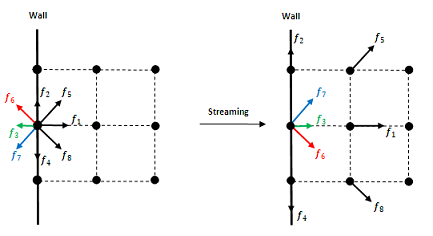
\includegraphics[width=\singleimagewidth]{figures/lbm/ongrid}
	\caption{Sketch of the D2Q9 nodes showing at the boundary the distribution functions that would come from neighbors outside the boundary (at the wall) are unknown (drawing from correspondence with Dr. Bao, billbao@cims.nyu.edu).}\label{fig:wall-lattice-bc}
\end{figure}


To treat velocity or pressure boundary conditions, the technique of Zou \& He is used.\cite{Zou1997} They proposed extending the bounce-back condition to the non-equilibrium distribution function in the direction normal to the boundary where $\vec{v}$ or $p$ is specified. The approach allows closure of the algebraic calculation of distribution functions when we have a known velocity or pressure (see Eqs.~\ref{eq:lbm2physical}). We note again that, in lattice units, determination of density is equivalent to determination of pressure \textit{via} the ideal gas pressure law. Zou \& He showed the approach provides second-order accurate results on these boundaries.\cite{Zou1997} 












\subsubsection{Thermal LBM}

Thus far the lattice-Boltzmann formulation has been shown to calculate mass and momentum transport of a fluid. But in the packed beds of fusion reactors, the transport of energy in the system is of utmost importance. To handle the thermal equations in the lattice-Boltzmann framework, we use the model of Guo\etal\cite{Guo2002} Guo\etal~introduced a second lattice upon which the distribution functions for temperature reside. The temperature distribution evolved with a coupling to the velocity distribution on the lattice solving the Navier-Stokes equations. The temperature was linked back to the Navier-Stokes lattice with a Boussinesq assumption that introduced a body force term to the fluid.\cite{Guo2002} Guo\etal~referred to their approach as the Coupled Lattice BGK (CLBGK) method. 

On the thermal lattice in the CLBGK method, the temperature is a passive scalar that is transported by the velocity (it is specified at each node corresponding to nodes from lattice solving the Navier-Stokes equations). Therefore, the density distribution functions on thermal lattices are in fact temperature distribution functions. The thermal lattice BGK equation is analogous to \Cref{eq:lbm-bgk} and written as,
\begin{equation}\label{eq:lbm-thermal-bgk}
	g_i(\vec{x}+\vec{c}_i, t + 1) = g_i(\vec{x},t) - \frac{1}{\tau_g}\left[g_i^\eq(\vec{x},t) - g_i(\vec{x},t)\right]
\end{equation}
where we have a second relaxation time for the thermal lattice, $\tau_g$. The temperature field is reconstructed via
\begin{equation}
	T = \sum_i^q g_i
\end{equation}

A multi-scale Champan-Enskog expansion of \Cref{eq:lbm-thermal-bgk} can show that it is equivalent to the temperature form of the continuous energy conservation equation.\cite{Guo2002} For the transport of the passive scalar, we can use a D3Q7 lattice which is sufficient to model the advection-diffusion of temperature.\cite{Latt2007,Parmigiani2011}, For such a lattice, the speed of sound is $c^2_{s,g} = \frac{1}{2}$. We use a linear equilibrium function for $g_i^\eq$,
\begin{equation}
	g_i^\eq = w_i T \left(1+\frac{\vec{c}_i\cdot\vec{u}}{c_{s,g}^2}\right)
\end{equation}

The thermal diffusivity (analogous to the viscosity in the momentum lattice) is 
\begin{equation}
	\alpha = c_{s,g}^2\left(\tau_{g} - \frac{1}{2}\right)
\end{equation}
% The coupling from temperature to density \textit{via} the Boussinesq assumption is done with the addition of a body force term, $g_i$ to the Navier-Stokes' BGK equation,
% \begin{equation}
% 	f_i^\eq = \rho(\vec{x},t)w_i\left[1+\frac{\vec{u}\cdot\vec{c}_i}{c_s^2} + \frac{(\vec{u}\cdot\vec{c}_i)^2}{2c_s^4} - \frac{\vec{u}^2}{2c_s^2} \right] + g_i
% \end{equation}
% where the body term is
% \begin{equation}
% 	g_i = -\frac{1}{2}\Delta t \alpha_i \vec{c}_i\cdot\vec{g}(T - T_0)
% \end{equation}

Thermal boundary conditions are handled \textit{via} a decomposition of the boundary nodes into equilibrium and non-equilibrium parts and the values of the node extrapolated from neighboring nodes. Details can be found in the paper by Guo\etal.\cite{Guo2002}


\subsection{Realizing LBM Models Computationally}
Because of the immensely simple implementation of no-slip boundary conditions for even the most complex geometry, the lattice-Boltzmann method was immediately seen as a powerful option of fluid modeling in porous networks. Chen \& Doolen review many of the major accomplishments of implementing LBM models which verified Darcy's Law, the Cozeny-Karman equation, and Brinkmann equation, among other efforts.\cite{Chen1998a} Pan\etal~evaluated the single-relaxation time BGK operator against models with multiple relaxation times as well as models with different implementationsi of fluid-solid interface boundary conditions -- among which was the bounce-back scheme we use here.\cite{Pan2006}

Here we will go through the practical application of the LBM approach as it will be used  to simulate the conjugate heat transfer of the helium purge gas through ceramic pebble beds. To summarize the method, there are two main objects required to define the structure of a lattice-Boltzmann model: a collision operator, $\Omega_i$, and the constants which define the scaffolding of the lattice.

The computational domain of the fluid is discretized into a Cartesian grid with regularized spacing, $\delta_x$, in every dimension. At each node are density functions, $f_i(\vec{x},t)$, which represent the density at that node (found at $\vec{x}$), traveling in the direction of $\vec{c}_i$ at a moment in time, $t$. The density distribution function evolves according to \Cref{eq:lbm-evolution}. It is helpful to look at the equation compartmentalized in the same manner it is handled computationally, thus we see the streaming and collision parts,
\begin{align}
	\underbrace{f_i(\vec{x}+\vec{c}_i, t + 1)  = f_i(\vec{x},t)}_\text{streaming}  + \underbrace{\Omega_i(\vec{x},t)}_\text{collision}
\end{align}

Conceptually the two steps of lattice evolution can be thought of as two distinct operations. First, the collision operator is calculated based only on each node's local information. Using the BGK approximation, given in \Cref{eq:bgk-operator}, the collision is calculated as
\begin{align}
	\Omega_i = -\frac{1}{\tau}\left[f_i(\vec{x},t) - f_i^\eq(\vec{x},t)\right]
\end{align}

Post-collision, in the streaming step, the information is passed from every node to its neighbors along the lattice directions shown in \Cref{fig:d3q19-lattice}. While the collision operation is exactly local, the streaming operation involves only nearest neighbors. After the streaming step, the nodes that lie along the boundary have the bounce-back scheme applied wherein distributions arriving at the boundary are reflected back to their incident directions.

Splitting the evolution of the distribution function into the two steps of collision and streaming, in addition to being a conceptual aid, is a natural partition of computational steps. In practice the algorithm proceeds as follows,\cite{Viggen2009}
\begin{enumerate}
	\item{using macroscopic properties of density and fluid velocity, the equilibrium distribution function is calculated at every node following \Cref{eq:equilib-dist-function},}
	\item{the BGK collision operator is calculated according to \Cref{eq:bgk-operator} to find the post-collision distribution of every node,}
	\item{information from each node streaming to neighboring nodes based on the evolution equation of \Cref{eq:lbm-evolution},}
	\item{updated macroscopic properties are found from the new distribution functions according to \Cref{eq:lbm2physical}.}
\end{enumerate}

It is worth stressing again that the lattice-Boltzmann collision calculations are completely local, with the streaming step requiring only nearest inter-node communication for updating distribution functions which lends the method to extremely efficient parallelization. 

% We now need a means of translating physical properties into lattice units. Then we can incorporate our pebble bed into the LBM computational space before LBM simulations of helium-pebble conjugate heat transfer can be performed.





\subsection{Physical to Lattice Units}\label{sec:physical-to-lattice}
In LBM one typically works with lattice variables -- differing from their physical counterparts simply through normalization. This is akin to achieving dynamic similarity in fluid mechanics experiments. I therefore will discuss the nondimensional form of governing equations and then translate the nondimensional values into lattice variables. We then see how tuning of some lattice variables will allow a sufficiently refined grid while still representing the physical system we are attempting to model. The notation of working with physical, nondimensional, and lattice variables can quickly become cumbersome. The convention I will adhere to is to use $\hat{\psi}$ for physical variables, $\psi^*$, or nondimensional variables, and simply $\psi$ for lattice variables.

Thus the Navier-Stokes equations, in physical units, for an incompressible fluid are
\begin{equation}
	\hat{\nabla}\cdot\hat{\vec{u}} = 0
\end{equation}
and
\begin{equation}
	\frac{\partial \hat{\vec{u}}}{\partial \hat{t}} + (\hat{\vec{u}}\cdot\hat{\nabla})\hat{\vec{u}} = -\frac{1}{\hat{\rho}_0}\hat{\nabla}\hat{p} + \hat{\nu}\hat{\nabla}^2\hat{\vec{u}}
\end{equation}

I nondimensionalize the length scale based on the average diameter of pebble in our system, the velocity by the superficial velocity of our inlet, and pressure and time on derived forms of these two variables,
\begin{subequations}
\begin{align}
	x^* &= \frac{\hat{x}}{\hat{d}_p} \\
	\vec{u}^* &= \frac{\hat{\vec{u}}}{\hat{|u|}_i} \\
	p^* &= \frac{\hat{p}}{\hat{\rho}_0\hat{|u|}_i^2}\\
	t^* &= \frac{\hat{t}}{\frac{\hat{d}_p}{\hat{\vec{u}}_i}}
\end{align}
\end{subequations}

Thus the nondimensional form of Navier-Stokes is the familiar,
\begin{subequations}\label{eq:non-dim-ns}
\begin{align}
	\nabla^* \cdot \vec{u}^* &= 0 \\
	\frac{\partial \vec{u}^*}{\partial t^*} + (\vec{u}^*\cdot\nabla^*)\vec{u}^* &= -\nabla^*p^* + \frac{1}{\Re}\nabla^{*2}\vec{u}^*
\end{align}
\end{subequations}

Note, too, that the physical limits of our system are describable in terms of the nondimensional units. In other words, if our system is $\hat{X}$ meters wide, the nondimensional width is $X^*=\frac{\hat{X}}{\hat{d}_p}$.  

% The last thing we need before converting the variables of \Cref{eq:non-dim-ns} into lattice units are the lattice spacing and lattice time step, $\delta_x$ and $\delta_t$. We will define the lattice spacing based on the resolution of our pebble diameter, as described above.

% The manner of description I will follow next will match the method in which the values are actually programmed in my DEM-to-LBM script. I begin by defining the pebble diameter, limits, and resolution ($\text{res}$); the script returns $\delta_x$, $N_x$, $N_y$, and $N_z$ where the $N$ values represent the total number of nodes in a given direction. 

Next, the dimensionless kinematic viscosity, $\nu^* = 1/\Re$, is converted into a lattice viscosity as
\begin{equation}\label{eq:fluid-nu}
	\nu = \frac{\delta_t}{\delta_x^2}\frac{1}{\Re}
\end{equation}
from which, we can finally calculate the relaxation time for our single-relaxation-time, D3Q19 lattice (calculated from \Cref{eq:lbm-viscosity-relaxation-time}) as,
\begin{equation}
	\tau_{ns} = \frac{\nu}{c_s^2} + \frac{1}{2}
\end{equation}
where the subscript $_{ns}$ denotes the relaxation time is specific for the fluid flow as described by the Navier-Stokes equations and the lattice speed of sound is $c_s^2 = \frac{1}{3}$.

To specify the velocity boundary condition (and similarly to convert our lattice velocity results back into physical values), we must have a translator between nondimensional and lattice velocities,
\begin{equation}\label{eq:lbm-u}
	\vec{u} = \frac{\delta_t}{\delta_x}\vec{u}^*
\end{equation}

Translating from physical to lattice units is done via,
\begin{equation}
	\vec{u} = \frac{\delta_t}{\delta_x}\frac{\hat{\vec{u}}}{\hat{|u|}_i}
\end{equation}

The spatial discretization of the lattice is defined in terms of the resolution of our sphere in the discretization process. The values of lattice spacing, $\delta x$, and the total lattice nodes are calculated as,
\begin{subequations}
\begin{align}
	\delta_x = \delta_y = \delta_z & = \frac{1}{\text{res}} \\
	N_x & = \text{res}\cdot X^* +1\\
	N_y & = \text{res}\cdot Y^* +1\\
	N_z & = \text{res}\cdot Z^*+1
\end{align}
\end{subequations}
where $\text{res}$ is defined as the number of nodes spanning the diameter of a pebble. 

The only lattice parameter not defined at this point is the lattice time step, $\delta_t$. In lattice-Boltzmann, $\delta_t$ and $\delta_x$ are linked \textit{via} the incompressibility constraint in the lattice. At the same time, from \Cref{eq:lbm-u}, the lattice velocity is directly related to the lattice time step size; and the magnitude of $\vec{u}$ may not be larger than the speed of sound on the lattice, $c_s$. The time step is further constrained when enforcing incompressibility of our fluid. The LB model is a quasi-compressible fluid solver which permits slight compressible regimes to enter the system to solve the pressure equation of the fluid. Compressibility effects will impact the numerical accuracy and should therefore be minimized. Compressibility effects scale like the square Mach-number, $\Ma^2$, and thus effects can be minimized by enforcing a small Mach number. In LBM, the lattice Mach number is simply,
\begin{equation}
 	\Ma = \frac{|\vec{u}_0|}{c_s}
\end{equation}
where $|\vec{u}_0| = \frac{\delta_t}{\delta_x}$. Thus to say the compressibility error scales like $\epsilon \sim \Ma^2$ is to say it scales like $\epsilon \sim \frac{\delta_t^2}{\delta_x^2}$. The compressibility error need not be smaller than the numerical error of the LBM method itself. As LB is second-order accurate\cite{succi2001lattice}, $\epsilon \sim \delta_x^2$, we can then determine the time step size relative to lattice spacing for which the two errors will be comparable in size,
\begin{align*}
	\frac{\delta_t^2}{\delta_x^2} &\sim \delta_x^2\\
	\rightarrow \delta_t &\sim \delta_x^2
\end{align*}

Also, because the lattice spacing is directly dependent on our chosen resolution, the requirement on time step is alternatively written as
\begin{equation}
	\delta_t \sim \frac{1}{\text{res}^2}
\end{equation}
which shows, similar to standard CFD solvers, the time step requirement shrinks rapidly as we attempt to more finely represent the pebbles with more and more nodes. Thus care must be taken to balance the resolution with the time step requirements.

In the LBM model, we only treat the energy as a passive scalar transported by the fluid motion (\textit{i.e.} we do not make the Boussinesq approximation to couple the fluid energy to momentum). The energy equation for the fluid in physical units is,
\begin{equation}
	\frac{\partial \hat{T}_f}{\partial \hat{t}} + \hat{\nabla}\cdot(\hat{\vec{u}}\,\hat{T}_f) = -\hat{\alpha}_f\hat{\nabla}^2\hat{T}_f
\end{equation}

The temperature will be nondimensionalized based on a characteristic temperature of volumetric heating,
\begin{equation}
	T^* = \frac{\hat{T} - \hat{T}_c}{\Delta \hat{T}}
\end{equation}
and the time and length scales are nondimensionalized as in the Navier-Stokes equations. Thus the nondimensional energy equation is
\begin{equation}\label{eq:non-dim-energy}
	\frac{\partial T^*_f}{\partial t^*} + \nabla^*(\vec{u}^*T^*_f) = \frac{1}{\Pe_f} \nabla^{*2}T^*_f
\end{equation}
where $\Pe$ is the Peclet number ($\Pe = \Re\cdot \Pr$).

To discretize the dimensionless energy system into the lattice, we recognize the similarities between \Cref{eq:non-dim-ns} and \Cref{eq:non-dim-energy} to directly write the lattice thermal diffusivity of the fluid as
\begin{equation}\label{eq:fluid-alpha}
	\alpha_f = \frac{\delta_t}{\delta_x^2}\frac{1}{\Pe_f}
\end{equation}

For the solid, the energy equation in dimensional units is
\begin{equation}
	\frac{\partial \hat{T}_s}{\partial \hat{t}} = \hat{\alpha}_s\hat{\nabla}^2\hat{T}_s + \frac{\hat{q}'''}{\hat{\rho}_s\hat{C}_{ps}}
\end{equation}

which similarly nondimensionalizes to,
\begin{equation}\label{eq:non-dim-energy-solid}
	\frac{\partial T^*_s}{\partial t^*} = -\alpha_s^* \nabla^{*2}T^*_s + Q^{'''*}
\end{equation}
where the dimensionless thermal diffusivity of the solid is $\alpha_s^* = \frac{\hat{\alpha_s}}{\hat{d}_p\hat{u}_i}$ and the dimensionless nuclear heating rate is $Q^{'''*} = \frac{\hat{q}'''\hat{d}_p}{\hat{u}_{i}\hat{\rho}_s\hat{C}_{ps}\Delta\hat{T}}$.

We can now directly write the lattice thermal diffusivity of the solid as
\begin{equation}\label{eq:solid-alpha}
	\alpha_s = \frac{\delta_t}{\delta_x^2}\frac{1}{\alpha_s^*}
\end{equation}

The lattice heat rate is $Q = \delta_tQ^{'''*}$

On the thermal lattice, we need only use a D3Q7 to satisfy isotropy, for which the lattice speed of sound is only $c_s^2 = \frac{1}{2}$ (I will refer to it as $c_{s,ad}$ to distinguish). On this lattice, we are solving the energy equation for both the fluid and solid, so each material has a unique relaxation time. I will refer to them as the advection-diffusion (ad) and conjugate (cj) relaxation times, for short. They are,
\begin{subequations}
\begin{align}
	\tau_{ad} &= \frac{\alpha_f}{c_{s,ad}^2} + \frac{1}{2} \\
	\tau_{cj} &= \frac{\alpha_s}{c_{s,ad}^2} + \frac{1}{2}
\end{align}
\end{subequations}
and the size of lattice spacing and time steps are equal to those of the Navier-Stokes lattice.

To summarize the unit conversion process described above, our lattice needs to be defined in terms of lattice spacing and time step. The physics of the system are encompassed in the relaxation time -- values which can be determined completely from lattice spacing and nondimensional values of the Reynolds, Peclet, and solid diffusivity values. Physical boundary conditions of velocity and temperature can be enforced in the lattice with translations into lattice variables as given above. 

Lattice diffusivity values given in \Cref{eq:fluid-nu}, \Cref{eq:fluid-alpha}, and \Cref{eq:solid-alpha}, respectively, are summarized together,
\begin{align*}
	\nu &= \frac{\delta_t}{\delta_x^2}\frac{1}{\Re} \\
	\alpha_f &= \frac{\delta_t}{\delta_x^2}\frac{1}{\Pe_f} \\
	\alpha_s &= \frac{\delta_t}{\delta_x^2}\frac{1}{\hat\alpha_s^*}
\end{align*}

From which we calculate relaxation times:
\begin{align*}
	\tau_{ns} &= \frac{\nu}{c_s^2} + \frac{1}{2} \\
	\tau_{ad} &= \frac{\alpha_f}{c_{s,ad}^2} + \frac{1}{2} \\
	\tau_{cj} &= \frac{\alpha_s}{c_{s,ad}^2} + \frac{1}{2}
\end{align*}

And relaxation parameters:
\begin{align*}
	\omega_{ns} &= \frac{1}{\tau_{ns}} \\
	\omega_{ad} &= \frac{1}{\tau_{ad}} \\
	\omega_{cj} &= \frac{1}{\tau_{cj}}
\end{align*}

%Perhaps not obvious from this discussion is that we could be free to model a fictitious fluid that allows for high numeric accuracy and stability provided that the nondimensional variables be translatable to proper physical ones.


\section{Numerical Implementation of LBM and DEM Coupling}\label{sec:lbm-solver}

As usual, the packing structure of our pebble bed is rendered with the code LIGGGHTS. Details of the software are described in \cref{sec:dem-solver}. The DEM solver is a highly parallel C++ code based on the Molecular Dynamics (MD) code LAMMPS.\cite{Plimpton1995} The translation between the DEM packing and LBM nodal network is done with Python scripts I created to discretize and digitize the `spherical' information of DEM into LBM. To solve the lattice-Boltzmann collision and streaming equations, we make use of the open-source code maintained by FlowKit Ltd named Palabos.\cite{Flow} The Palabos library provides an interface for quick implementation of lattice-Boltzmann models in C++. Implemented models include the BGK and thermal flows with the Boussinesq approximation, among many others. The lattices available are the common grids of D2Q9, D3Q13, D3Q15, D3Q19, or D3Q27. Zou/He, periodic, and bounce-back conditions are built into the LB kernel; implementation of Dirichlet or Neumann conditions with velocity or pressure are also available. The software is freely available under the terms of the open-source AGPLv3 license.\cite{FreeSoftwareFoundationInc.2007} All mentioned models and ingredients are parallelized with MPI, including the I/O operations that are implemented in terms of MPI’s Parallel I/O API.









\section{DEM Mapping to LBM \& Realizing Proper Hydrodynamics}
Unlike the dynamic coupling between DEM and the volume-averaged CFD where information passed back and forth between fluid and particle, in the LBM construction I am simply translating a static packing structure from DEM into the LBM framework. The lattices of the LBGK solver use equally spaced nodes that discretize our volume into regular spacing. The pebble data from DEM is mapped onto the LBM nodes with a script \textit{via} knowledge of the centroid and radius of each pebble. To demonstrate, in \Cref{fig:dem-2-lbm-example1}, we have a sketch of the outline of a two-dimensional slice of a pebble projected onto a section of an LBM lattice. If the distance from a node to the centroid is less than pebble radius, the node is assigned as solid. All other nodes are assigned as fluids.

\begin{figure}[ht]
	\centering
	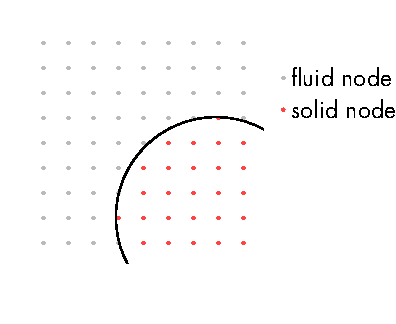
\includegraphics[width=\singleimagewidth]{figures/lbm/dem-to-lbm-mapping.pdf}
	\caption{An example of the mapping process from DEM to LBM structures. Nodes are assigned as fluid or solid based on relative location of pebble centroid and radius. Here we have a resolution of 9 (\textit{i.e.} 9 nodes per pebble diameter).}\label{fig:dem-2-lbm-example1}
\end{figure}

\begin{figure}[ht]
	\centering
	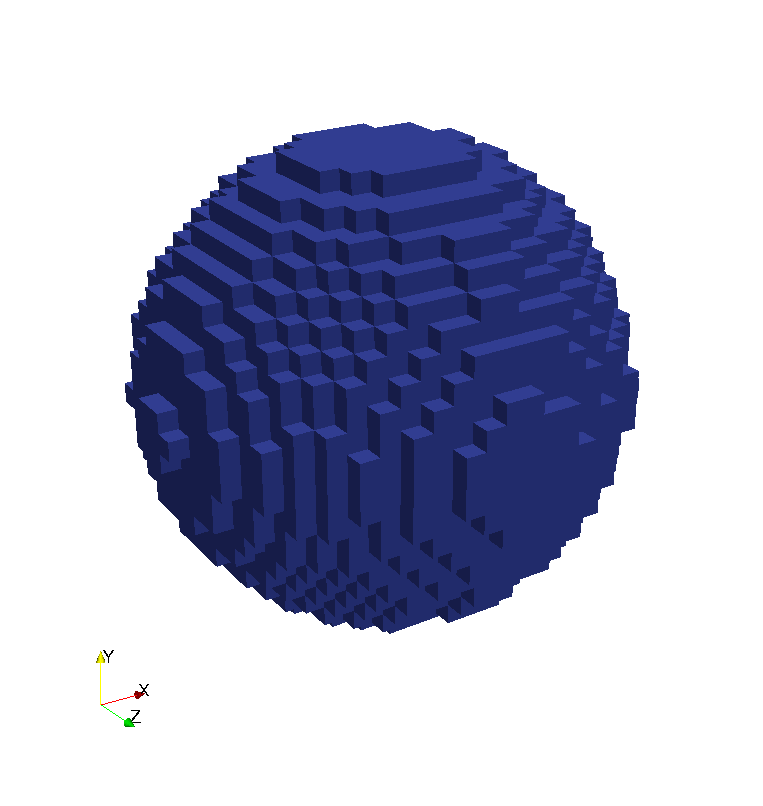
\includegraphics[width=\doubleimagewidth]{figures/lbm/lbm-pebble-res25.png}
	\caption{A three-dimensional DEM pebble as imported into the LBM lattice with a resolution of 25.}\label{fig:dem-2-lbm-example2}
\end{figure}

In the example of \Cref{fig:dem-2-lbm-example1}, the resolution is only 9. Thus 9 nodes are needed to span the diameter of a single pebble and the lattice spacing is $\delta_x = 1/9$. In the second example shown in \Cref{fig:dem-2-lbm-example2}, we see an individual pebble in three dimensions that has been mapped onto the LBM nodes with a resolution of 25 (thus $\delta_x = 1/25$). The trade-off between small lattice spacing is the ability to resolve the spherical surface of the pebble, stability, and even the ability to resolve a proper packing fraction in the pebble bed. 







\FloatBarrier
\subsection{Consistency of Packing Fraction in Digitization}
In the process of digitizing DEM onto lattice sites, the size of the sphere is often over-represented and the LBM lattice does not faithfully reproduce the correct void fraction from DEM. In order to capture proper macroscopic values of porosity on the lattice sites, a radius-reduction factor was introduced into the digitization process. Radii mapped into LBM are then $r_{lbm} = k r_{dem}$. The effects of the radius reduction factor can be seen in \Cref{fig:2d-dem-lbm-mapping}, where the void fraction is calculated as discussed below.

\begin{figure}[ht]
        \centering
        \begin{subfigure}[b]{0.2\textwidth}
                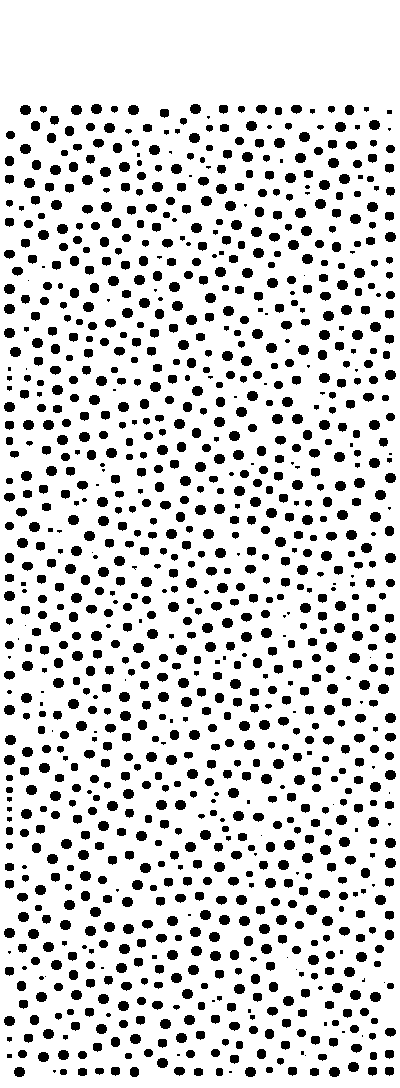
\includegraphics[width=\textwidth]{figures/lbm/2d-res20-k050.png}
                \caption{$\phi = 0.181$ in pebble bed section with $k = 0.50$.}
                \label{fig:2d-res20-k050}
        \end{subfigure}%
        ~
        \begin{subfigure}[b]{0.2\textwidth}
                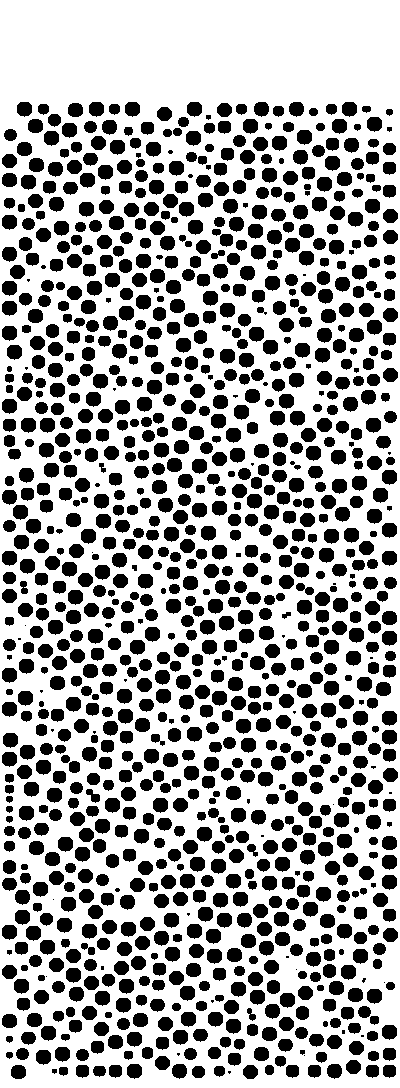
\includegraphics[width=\textwidth]{figures/lbm/2d-res20-k075.png}
                \caption{$\phi = 0.389$ in pebble bed section with $k = 0.75$.}
                \label{fig:2d-res20-k075}
        \end{subfigure}%
        ~
          %add desired spacing between images, e. g. ~, \quad, \qquad, \hfill etc.
          %(or a blank line to force the subfigure onto a new line)
        \begin{subfigure}[b]{0.2\textwidth}
                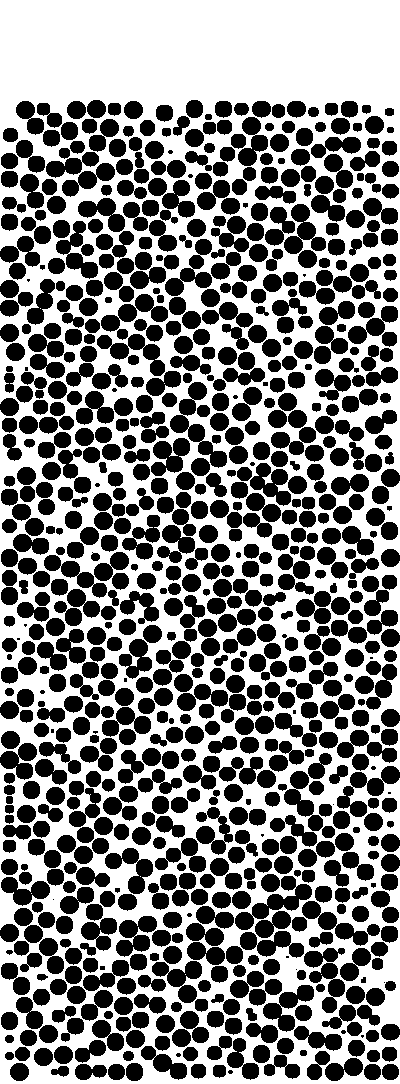
\includegraphics[width=\textwidth]{figures/lbm/2d-res20-k090.png}
                \caption{$\phi = 0.555$ in pebble bed section with $k = 0.90$.}
                \label{fig:2d-res20-k090}
        \end{subfigure}
        ~
        \begin{subfigure}[b]{0.2\textwidth}
                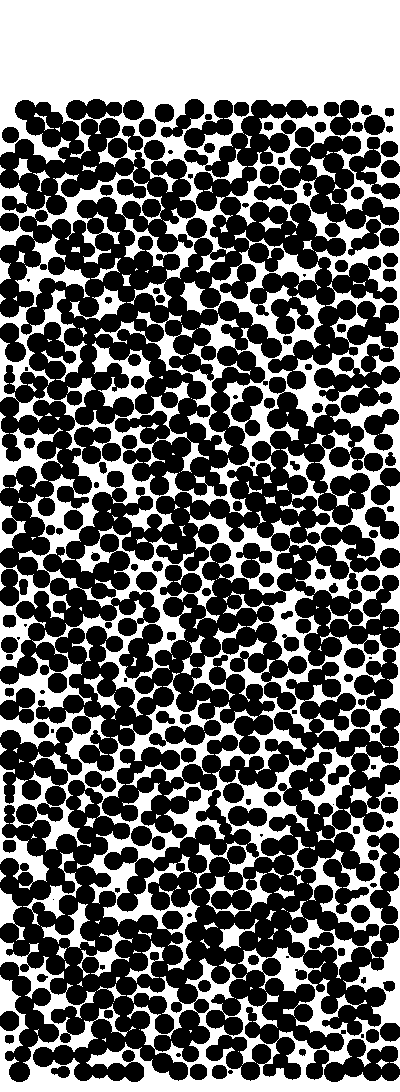
\includegraphics[width=\textwidth]{figures/lbm/2d-res20-k100.png}
                \caption{$\phi = 0.667$ in pebble bed section with $k = 1.00$.}
                \label{fig:2d-res20-k100}
        \end{subfigure}
        \caption{For a given resolution, the scaling parameter $k$ will result in different packing fractions. These mappings were generated from a pebble bed with $\phi =0.64$; only a specific $k$ will yield that void fraction after mapping into LBM.}\label{fig:2d-dem-lbm-mapping}
\end{figure}


A digital void fraction for each mapping was measured numerically by comparing the number of white pixels to black pixels in each bitmap slice,
\begin{equation}
	\phi_{d,j} = \frac{N_\text{black}}{N_\text{white}+N_\text{black}}
\end{equation}

Then the total digital packing fraction of the ensemble, as mapped into LBM, is simply
\begin{equation}
	\phi_d = \frac{1}{J}\sum_j^J\phi_{d,j}
\end{equation}

where there are $J$ total slices. For example, we see in \Cref{fig:dem-2-lbm-packing-fraction} a plot of the digital packing fraction moving through a particular pebble bed. Digital packing fractions changed as a function of the radius-reduction factor and can be seen in \Cref{fig:2d-dem-lbm-mapping}. The DEM packing from which these slices originated was a $\phi =0.64$ initial packing of \Cref{sec:isfnt-12}.

\begin{figure}[h]
	\centering
	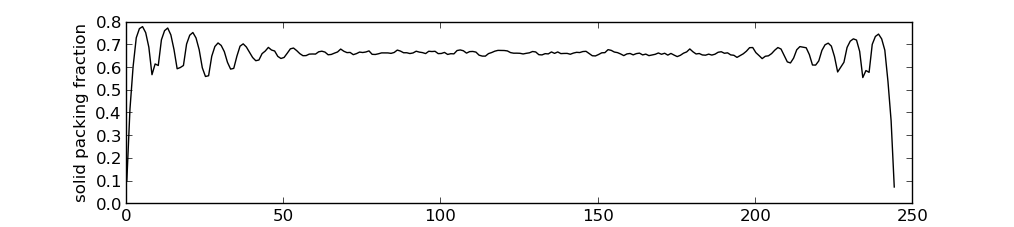
\includegraphics[width=\textwidth]{figures/lbm/palabos_packing_fraction}
	\caption{The digital packing fraction was measured at all slices through the height of the pebble bed. When the average value equaled the expected value, the mapping from DEM to LBM was considered consistent.}\label{fig:dem-2-lbm-packing-fraction}
\end{figure}






\subsection{Pore Size Effects on Hydrodynamics}
To model proper hydrodynamics with the lattice-Boltzmann method there are still several measures the lattice must satisfy. Several numerical experiments by Succi\etal~have shown proper hydrodynamics of Pouiselle flow in channels requires 4 lattice sites for fluid in pores of porous media.\cite{succi2001lattice} When spherical packings are digitized onto LBM lattices, constricted pores are consistently observed when resolutions are low. Taking DEM packings from \Cref{sec:isfnt-12}, we analyze the pore size distributions of different resolutions. The important pore size for a flow in the $x$-direction is the transverse $y$-$z$-plane. Thus taking a digitized bitmap of the $\phi = 0.64$  DEM packings, we measure the pore size sweeping along the $y$- and $z$-axes to generate \Cref{fig:res-pore-sizes} for various resolutions. 

\begin{figure}[h]
    \centering
    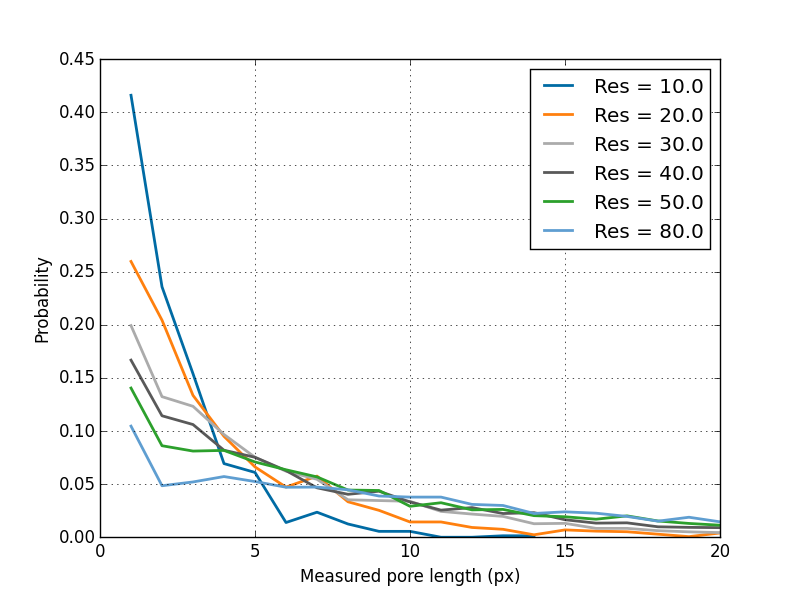
\includegraphics[width=0.75\textwidth]{figures/lbm/res-pore-sizes}
    \caption{Normalized histogram of pore sizes with increasing resolution. Hydrodynamic fidelity is violated with average pore sizes less than 4 nodes on the LBM lattice.}\label{fig:res-pore-sizes}
\end{figure}

\begin{figure}[h]
    \centering
    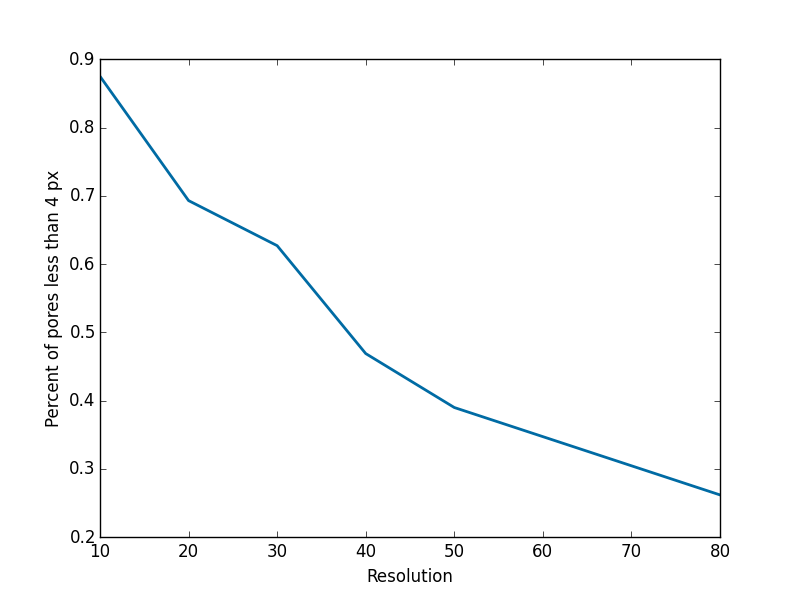
\includegraphics[width=0.75\textwidth]{figures/lbm/percent-pores-under-4px}
    \caption{For small resolutions, the number of pore openings smaller than 4 lattice nodes is 87.5\%. Increasing the resolution to 80 reduces this percentage to 26.2\%.}\label{fig:percent-pores-under-4px}
\end{figure}

\Cref{fig:percent-pores-under-4px} shows the percentage of pore openings in the lattices that are less than the 4 nodes recommended for proper hydrodynamics. Adhering to Succi's criteria of 4 pixel-wide pore opening minimums, it is obvious that the lattice resolution of 10 is unacceptable in terms of faithful reproduction of packed bed flow hydrodynamics: nearly 90\% of the pores in the lattice are less than 4 nodes wide. It is less evident if the violation of 4-node recommendation of other resolutions are allowable. 

The Knudsen number, the ratio of a gas's mean free path, $\lambda_{mfp}$, to a characteristic geometric length of the system, $L$, 
\begin{equation}
\Kn = \frac{\lambda_{mfp}}{L}
\end{equation}
is a key nondimensional parameter indicating when continuum assumptions, free molecule solutions, or rarefaction take place in a gas flow. The mean free path for an ideal gas can be calculated as
\begin{equation}
\lambda_{mfp} = \frac{\mu}{\rho}\sqrt{\frac{\pi M}{2k_bT}}
\end{equation}
where viscosity, $\mu$, and density, $\rho$, are temperature-dependent. $M$ is molecular mass, $k_b$ the Boltzmann constant, and $T$ absolute temperature.

A classification of flow regimes dictates that must be $\Kn < 10^{-2}$ for the continuum assumption to hold.\cite{karniadakis2006microflows} The Knudsen number is calculated as a function of pore size and temperature for helium in \Cref{fig:Knudsen_limits}. To satisfy the $\Kn$ criteria for continuum modeling, pore sizes must be larger than \SI{50}{\micro\meter} for helium at \SI{400}{\celsius} and greater than \SI{100}{\micro\meter} at \SI{900}{\celsius}. In packed beds of spheres, a large range of pore sizes appears. Near the contact points of two pebbles, pore sizes can be extremely small. Simultaneously, pore sizes between some pebbles in the packing can be on the order of pebble diameters. 

\begin{figure}[ht]
    \centering
    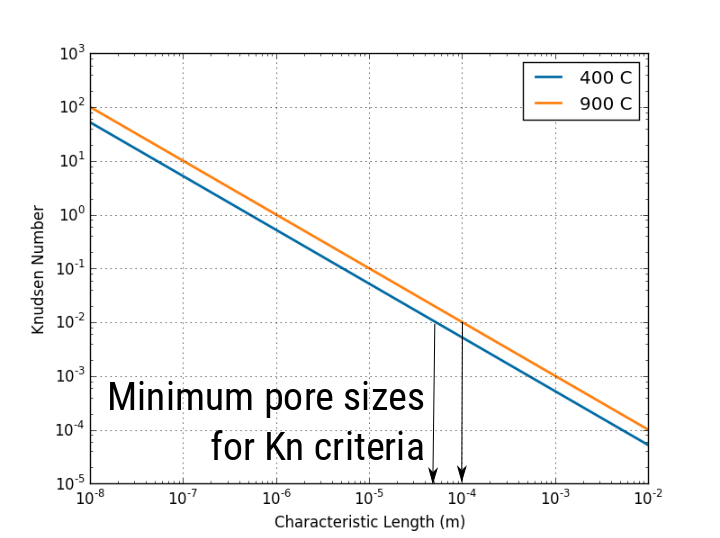
\includegraphics[width=0.75\textwidth]{figures/lbm/Knudsen_limits}
    \caption{Knudsen number for helium at \SI{400}{\celsius} and \SI{900}{\celsius} as a function of characteristic pore size.}\label{fig:Knudsen_limits}
\end{figure}

We can measure pore size distribution from a digitized DEM packing structure with an extremely fine resolution, res = \num{10000}. The pore size is converted into micro-meters from the translation between resolution and pebble diameter (resolution = pixels/mm). The result is shown in \Cref{fig:res10000-pore-size-distributions}.

\begin{figure}[ht]
    \centering
    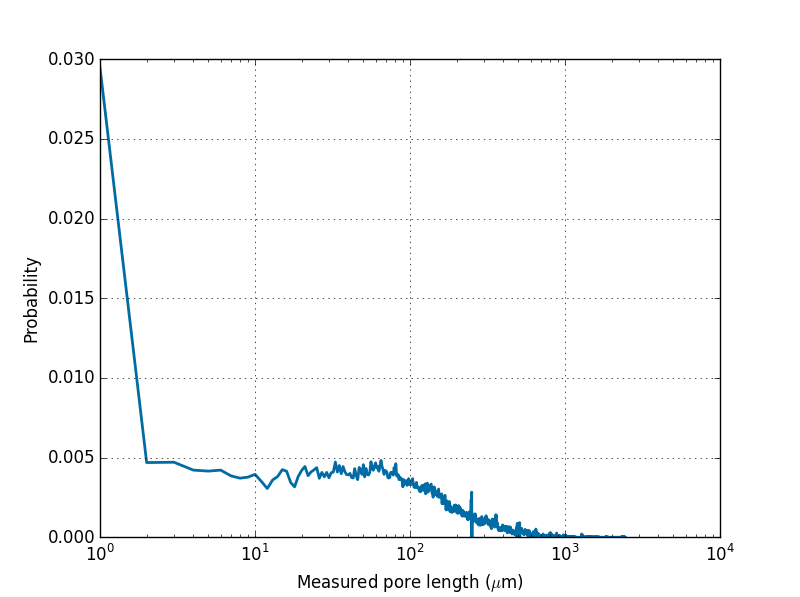
\includegraphics[width=0.75\textwidth]{figures/lbm/res10000-pore-size-distributions}
    \caption{Measured pore sizes from digitized DEM packings at $\phi = 0.64$, determined from a lattice with res = \num{10000}.}\label{fig:res10000-pore-size-distributions}
\end{figure}

Analysis of the pore size distribution tells us that this packed bed has 41.2\% of its pores smaller than \SI{100}{\micro\meter} and 22.5\% of the pore openings are smaller than \SI{50}{\micro\meter}. In other words, based on the Knudsen number of helium, at \SI{400}{\celsius}, nearly a quarter of the gaseous space in the pebble bed is violating the assumption necessary for continuum treatment of the fluid. As the temperature increases to \SI{900}{\celsius}, almost half of the gaseous space is in violation of the continuum assumption. 

The issue of violating Knudsen criteria in heated packed beds is left for future consideration. The main conclusion to draw is that Succi criteria of 4 nodes per pore opening being the minimum to satisfy hydrodynamic fidelity in LBM may not be completely applicable to packed beds which, themselves, are not satisfying criteria for being handled by continuum models. Comparing the outcome of this Knudsen analysis with the pore sizes of \Cref{fig:percent-pores-under-4px}, and perhaps even a resolution as low as 20 may still have an acceptable level of pore size distribution in light of Knudsen criteria violation.



\subsection{Parametric Study with Resolution and Packing Fractions}
We now apply LBM models to a variety of DEM-generated pebble beds to find an optimum resolution which yields both tractable models in terms of computational time as well as faithfulness of fluid flow physics.

Packing fraction and resolution of slices have a direct impact on lattice stabilities and faithful reproduction of hydrodynamics on the lattice. To study stability we consider several two-dimensional slices from a three-dimensional packing, such as the slices shown in \Cref{fig:2d-dem-lbm-mapping}. Lattices were generated with varying values of both radius reduction factor, $k$, and resolution, $\res$. Using simple boundary conditions of no-slip on the left and right walls, a Neumann boundary condition at the outlet (top) and constant velocity at the inlet (bottom), all latices were tested to find the stability of the resolutions and packings. To determine if a steady-state condition was reached, the velocity of the entire lattice was integrated. The value has units of $\psi = [m/s][lu^2]$, with dimensionless lattice spacing units. The value of $\psi$ is plotted in \Cref{fig:2d-lbm-settings-velocity}; we see a steady-state velocity is reached in all of the low-packing fraction lattices. As the packing fraction increased, following the increase of $k$, we see the system velocity slowly becomes unstable. When $k$ = 0.9, with a packing fraction of $\phi = 0.555$, the system approximately linearly increases into unstable values. Note, for the case when $k=1$, the density calculated in this system blew up to $\infty$ in less than 300 steps, so the velocity profile does not have a chance to demonstrate the unstable increase. For that bed, the packing fraction was high enough that there was not a continuous path available between inlet and outlet.

\begin{figure}[ht]
    \centering
    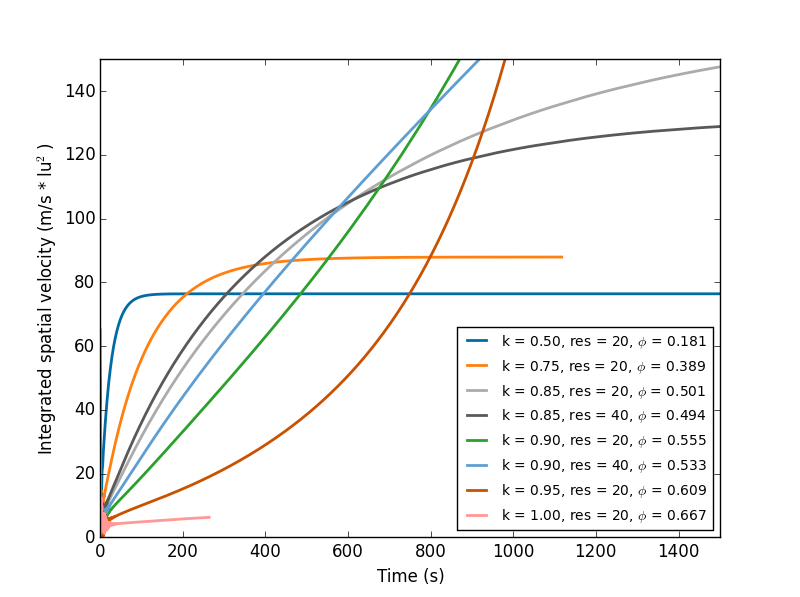
\includegraphics[width=0.75\textwidth]{figures/lbm/2d-lbm-settings-velocity}
    \caption{Integrated system velocity shows stable lattice configurations in two dimensions.}\label{fig:2d-lbm-settings-velocity}
\end{figure}

The two-dimensional study shows settings that lead to a stable lattice but, because of the limitations of two-dimensional lattices, such as rapid instability in such cases as $k=1$, an additional study was done on a scaled-down pebble bed in three-dimensions (temporarily without consideration for the error of the modeled hydrodynamics). The simplified system considers a pebble bed with width of $6d_p$, periodic depth of $1d_p$, and height of approximately $6d_p$. The pebble bed is discretized using the same numeric schemes and loaded onto three-dimensional lattices. The pebble bed, as visualized from DEM data, is shown in \Cref{fig:3d-bed-lbm}. When the simplified pebble bed is mapped onto discrete LBM nodes, we see the effects of resolution in \Cref{fig:3d-dem-lbm-mapping}. Here we have chosen resolutions of 10, 20, and 40, respectively. For each resolution, the coarseness of discretization requires varying radius reduction factors in order to achieve a consistent digital packing fraction; k = 0.92, 0.947, and 0.97, respectively. Details of the lattices are given below in \Cref{tab:3d-simp-lbm-parameters}.

\begin{figure}[ht]
    \centering
    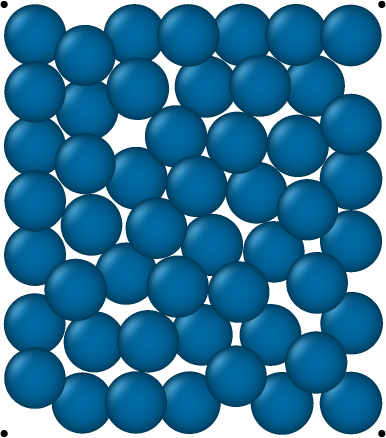
\includegraphics[width=0.3\textwidth]{figures/lbm/3d-bed}
    \caption{Simplified three-dimensional pebble bed, packing generated with DEM.}\label{fig:3d-bed-lbm}
\end{figure}

\begin{figure}[ht]
        \centering
        \begin{subfigure}[b]{0.3\textwidth}
                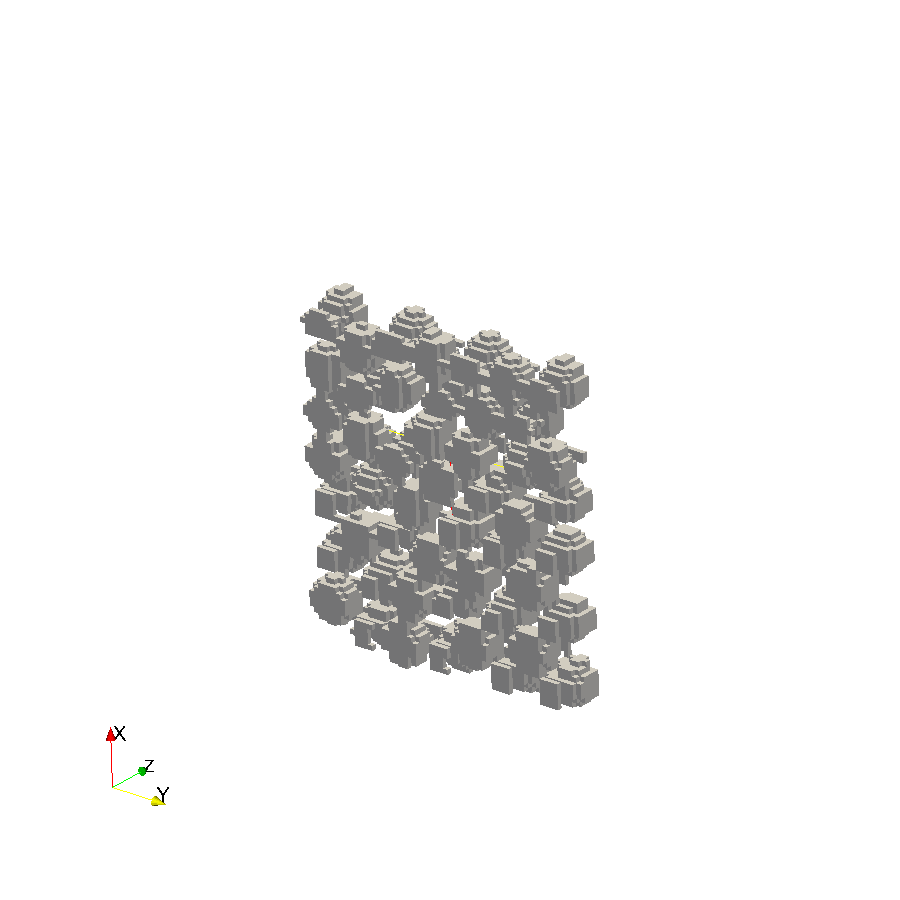
\includegraphics[width=\textwidth, trim={200pt, 150pt, 200pt, 200pt},clip]{figures/lbm/k092res10}
                \caption{Pebble bed with $k = 0.92$, $\res = 10$.}
                \label{fig:k092res10}
        \end{subfigure}%
        ~
        \begin{subfigure}[b]{0.3\textwidth}
                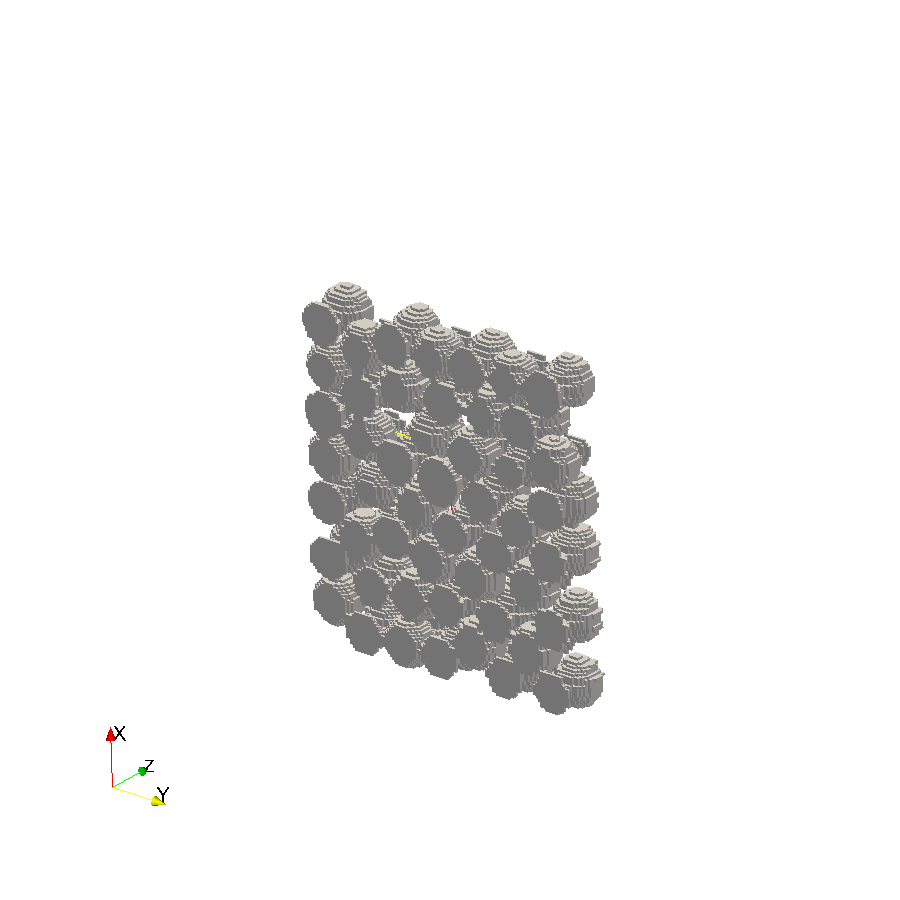
\includegraphics[width=\textwidth, trim={200pt, 150pt, 200pt, 200pt},clip]{figures/lbm/k0947res20}
                \caption{Pebble bed with $k = 0.947$, $\res = 20$.}
                \label{fig:k0947res20}
        \end{subfigure}%
        ~
          %add desired spacing between images, e. g. ~, \quad, \qquad, \hfill etc.
          %(or a blank line to force the subfigure onto a new line)
        \begin{subfigure}[b]{0.3\textwidth}
                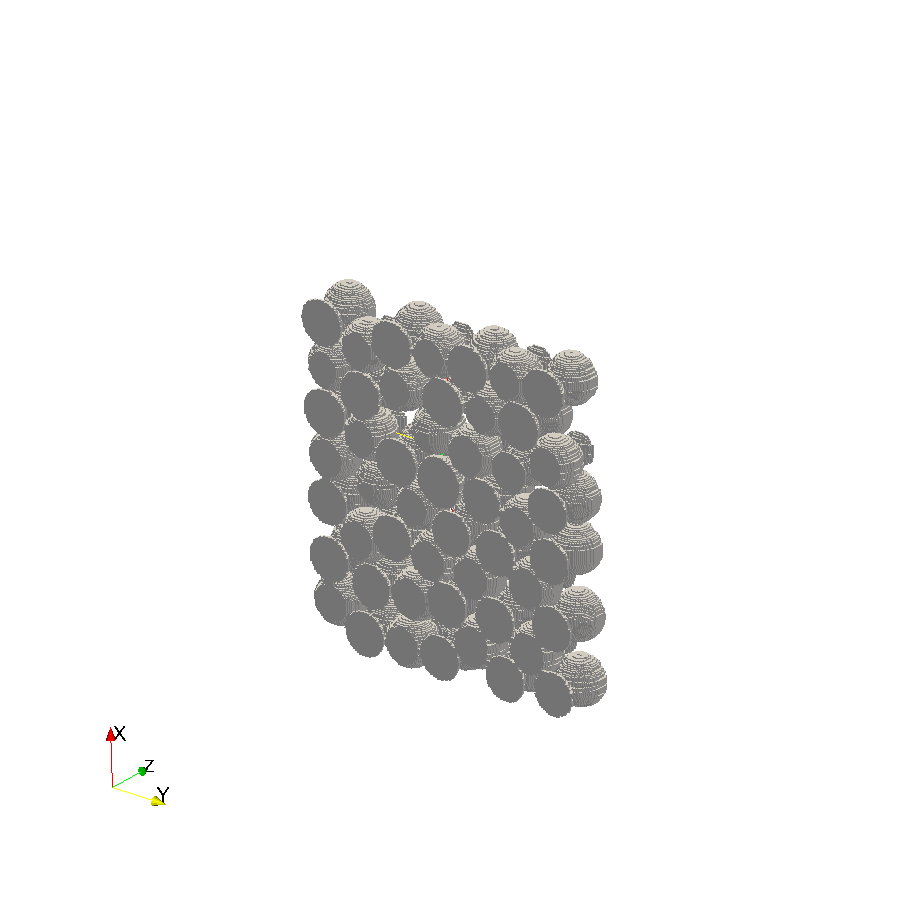
\includegraphics[width=\textwidth, trim={200pt, 150pt, 200pt, 200pt},clip]{figures/lbm/k097res40}
                \caption{Pebble bed with $k = 0.97$, $\res = 40$.}
                \label{fig:k097res40}
        \end{subfigure}
        \caption{For a specified packing fraction, 62.4\%, different resolution lattices require different radius scaling factors. The increased resolution is seen in increasing accuracy of spherical modeling on the discretized lattice.}\label{fig:3d-dem-lbm-mapping}
\end{figure}

\begin{figure}[ht]
    \centering
    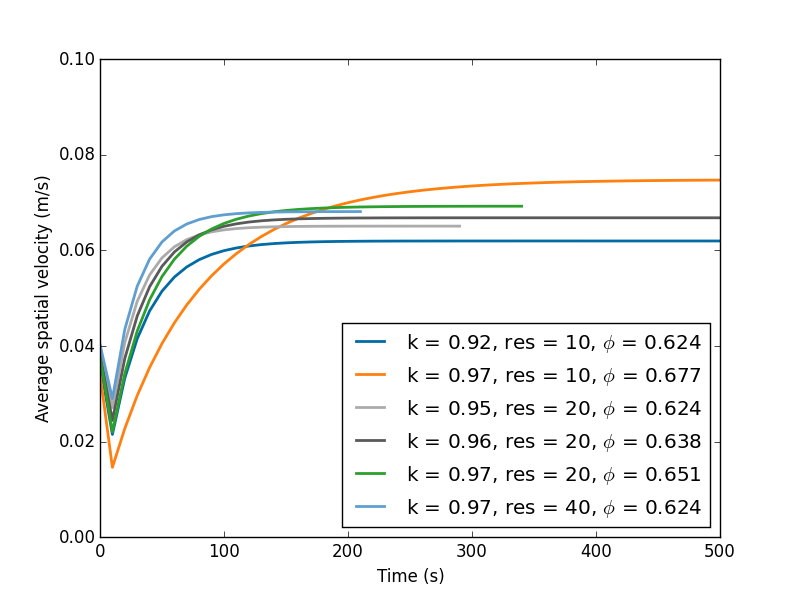
\includegraphics[width=0.75\textwidth]{figures/lbm/3d-lbm-settings-velocity}
    \caption{Averaged system velocity shows pebble beds with the same digital packing fraction and different resolutions will have different average system velocities.}\label{fig:3d-lbm-settings-velocity}
\end{figure}

In \Cref{fig:3d-lbm-settings-velocity}, the lattices shown in \Cref{fig:3d-dem-lbm-mapping} and others have their overall average velocity plotted. In this case, the magnitude of steady-state velocity is important so the integrated velocity has been divided by the total fluid space in the simulation. We see from \Cref{fig:3d-lbm-settings-velocity} that a lattice with the same packing fraction will have slightly different rates at which steady-state is approached. 

\begin{figure}[ht]
    \centering
    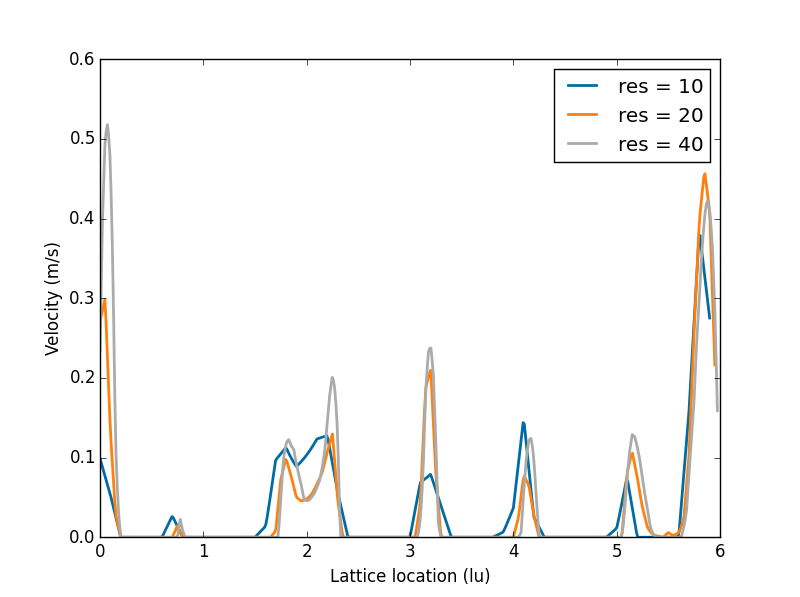
\includegraphics[width=0.75\textwidth]{figures/lbm/3d-bed-v-profiles}
    \caption{Low resolution lattices show qualitatively similar behavior but have insufficient resolution to capture jet velocity magnitudes.}\label{fig:3d-bed-v-profiles}
\end{figure}

At a location along the axial midpoint, velocity profiles across the pebble bed are shown in \Cref{fig:3d-bed-v-profiles}. The velocity jets in the near-wall region, caused by low packing fraction from ordered packing, are not well-captured by the low resolution ($\res = 10$) lattice. Other features of velocity are qualitatively seen in the low resolution packing, such as the velocity near $x = 2$~lu, but the $\res=20$ shows much greater correspondence with the profiles predicted by the highest resolution packing. 

Considerations of the velocity in the packed bed are important because the impact of tortuous velocity pathlines are what we seek to understand with implementation of the DEM-LBM study. However, hydrodynamically, an important measure of the physical fidelity of the packing simulation is the pressure drop across the bed. In \Cref{fig:3d-study-pressure-drop}, the pressure drop between inlet and outlet as a function of time are given for the three packings with equal packing fraction (the beds of \Cref{fig:3d-dem-lbm-mapping}). The pressure drop predicted by the Kozen-Carman relationship is approximately \SI{66}{\pascal}. The steady state value of the $\res=40$ lattice is \SI{61}{\pascal}. The lower resolution, $\res=20$, lattice comes close to the KC prediction; the steady-state pressure drop is \SI{64}{\pascal}. The lowest resolution pebble bed lattice is unstable and the density blows up shortly after \SI{200}{\sec}.

The last aspect to consider in the execution of the LBM model is the duration of a complete simulation. The last row in \Cref{tab:3d-simp-lbm-parameters} shows the product of total timesteps (to reach 200 s) and total lattice nodes. Assuming a perfect scalability of the simulation, this value is approximately the number of calculations performed to solve for steady-state on the lattice. Normalizing against the $\res=10$ lattice, we see that it requires 16 times longer to run the $\res =20$ lattice and more than 255 times longer to run the $\res = 40$ lattice. The same scaling rules will apply to the full pebble bed lattices that we wish to study. Thus, like most models of packed beds, we are forced to concede some accuracy in physics of the model for simplifications that allow reasonable computational times. For this reason, we conclude that the $\res = 20$ lattice, with $k$ chosen to satisfy digital porosity, is the appropriate setting to continue pebble bed simulations. The $\res = 20$ lattice had reasonable accuracy on hydrodynamic measurements of pressure drop and showed acceptable ability to capture features of the flow velocity such as the near-wall jets.

\begin{figure}[ht]
    \centering
    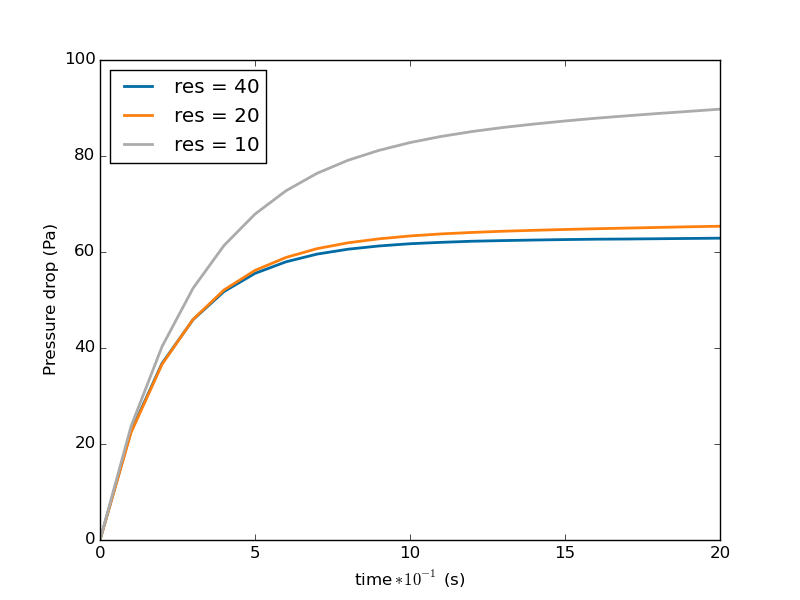
\includegraphics[width=0.75\textwidth]{figures/lbm/3d-study-pressure-drop}
    \caption{Pressure drops across the simplified pebble bed approaching steady-state in time. The low resolution pebble bed greatly over-predicts the pressure drop. Increased resolution appears to converge to approximately \SI{61}{\pascal}.}\label{fig:3d-study-pressure-drop}
\end{figure}

\begin {table}[ht] %
\caption{Comparison of lattice parameters for simplified pebble bed model.}
\label{tab:3d-simp-lbm-parameters} \centering %
\begin{tabular}{@{}lccc@{}}
\toprule %
	$\res$   &   10  &   20    &   40  \\\midrule
	$N_x$   &   60  &   120 &   240 \\
	$N_y$   &   10  &   20  &   40 \\
	$N_z$   &   138 &   276 &   553 \\
	$N_\text{tot}$  &   \num{82.8e3}     &   \num{662.4e3}    & \num{5308.8e3} \\
	$\omega_{ns}$     &   1.131   &   0.789   &   0.491   \\
	$\delta_x$  &   0.1     & 0.05  & 0.025 \\
	$\delta_t$  & 0.001     &   0.0005  & 0.00025   \\
	$N_t$   &   \num{200e3} &    \num{400e3}  & \num{800e3} \\
	$N_\text{tot} \times N_t$ & \num{16.6e9} & \num{264.9e9}     & \num{4247.0e9} \\\bottomrule
\end{tabular}
\end{table}


\FloatBarrier
%%%%%%%%%%%%%%%%%%%%%%%%%%%%%%%%%%%%%%%%%%%%%%%%%%%%%%%%%%%%%%%%%%%%%%%%%%%%%%%%%%%%%%%%%%%%%%%%%%%%%%%%%%%%
%%%%%%%%%%%%%%%%%%%%%%%%%%%%%%%%%%%%%%%%%%%%%%%%%%%%%%%%%%%%%%%%%%%%%%%%%%%%%%%%%%%%%%%%%%%%%%%%%%%%%%%%%%%%
%
% new section
%
%%%%%%%%%%%%%%%%%%%%%%%%%%%%%%%%%%%%%%%%%%%%%%%%%%%%%%%%%%%%%%%%%%%%%%%%%%%%%%%%%%%%%%%%%%%%%%%%%%%%%%%%%%%%
%%%%%%%%%%%%%%%%%%%%%%%%%%%%%%%%%%%%%%%%%%%%%%%%%%%%%%%%%%%%%%%%%%%%%%%%%%%%%%%%%%%%%%%%%%%%%%%%%%%%%%%%%%%%
\section{Summary of LBM Modeling Development}
The lattice-Boltzmann method of modeling fluid flow was introduced and its merits for application to porous flow discussed. We have shown a method for mapping data of packing structures, generated in DEM, onto nodes of lattices solving momentum/mass and energy conservation with collision-streaming operations of the lattice-Boltzmann method. The LBM approach was chosen in place of finite element or finite volume methodology because of, firstly, the extreme ease with which boundary conditions can be applied inside the highly complex packing structure of ceramic pebble beds; enforcing no-slip conditions on complex geometry is trivially realized with bounce-back rules on distribution functions. Furthermore, discretization of fluid domains in lattice-Boltzmann frameworks requires no special meshing in the highly-skewed regions near contacting pebbles, such as is necessary with standard CFD/FEM solvers. The multi-relaxation-time lattices for momentum and energy offer complete modeling of complex geometry and conjugate heat transfer with far less computational overhead compared to FEM models.

We also showed that proper selection of lattice properties can lead to stable solutions that are also faithful to the macroscopic fluid mechanics being modeled. Consistency in packing structure representation is maintained between DEM and LBM through modification of pebble radii when mapped on LBM voxels; accomplished through measurements of digital packing fraction in LBM lattices. We then considered the effects of grid sizing and resolution on stability of packed bed simulations. For densely packed beds, we found a resolution of 20 pixels/nodes per pebble diameter was sufficient for results that were: stable, capable of reproducing correct hydrodynamics, and computationally tractable.